\section{Requerimientos funcionales}\label{sec:requerimientosFuncionales}

\subsection{Formato de historias de usuario}
Los requerimientos funcionales fueron especificados a través de las historias de usuario siguiendo el siguiente formato que cumple con el definition of ready:

\begin{itemize}
    \item \textbf{Como:} Esta parte identifica quién es el usuario o rol específico que se beneficiará de la funcionalidad.
    \item \textbf{Quiero:} Aquí se describe la acción, tarea o funcionalidad que el usuario desea realizar. Debe ser una acción concreta y específica que permita 
    al usuario alcanzar un objetivo o resolver un problema.
    \item \textbf{Para:} Esta parte explica la razón o el beneficio que el usuario obtendrá al realizar la acción. Responde a la pregunta de por qué esta funcionalidad es 
    importante para el usuario.
\end{itemize}

A su vez, se utilizó el siguiente formato de escenarios para los criterios de aceptación:

\begin{itemize}
    \item [Nombre de escenario]
    \item \begin{itemize}
        \item Dado [un contexto],
        \item Cuándo [evento],
        \item Entonces [resultado]
    \end{itemize}
\end{itemize}


\subsection{Priorizacion de historias de usuario}

Este proceso se llevó adelante utilizando las reglas de priorización MoSCoW que es una técnica utilizada para categorizar y priorizar los requerimientos o funcionalidades en un proyecto. El acrónimo 
MoSCoW representa cuatro categorías principales:

% generar una lista numerada
\begin{enumerate}
    \item \textbf{Must have (Debe tener):} Estos son los requisitos críticos que son esenciales para el éxito del proyecto. Sin ellos, el proyecto no puede funcionar adecuadamente.
    \item \textbf{Should have (Debería tener):} Son requisitos importantes, pero no esenciales. Aunque su ausencia no detendrá el proyecto, sí afectaría significativamente su valor o eficiencia.
    \item \textbf{Could have (Podría tener):} Son requisitos deseables que, si se implementan, añadirán valor al proyecto, pero que se pueden considerar prescindibles si hay limitaciones de tiempo o recursos.
    \item \textbf{Won't have (No tendrá):} Requisitos que se han identificado pero que no se incluirán en la entrega actual del proyecto. Pueden ser considerados para futuras iteraciones.
\end{enumerate}

Esta clasificación se realizó en la etapa de Conversation, donde se establece un diálogo cercano y colaborativo con el cliente para definir y acordar los detalles de las historias de usuario. 
Durante esta fase, se discuten las necesidades, expectativas y prioridades del cliente, y se clarifican los requisitos de cada historia de usuario.\\
El propósito de esta conversación es asegurarse de que el equipo de desarrollo y el cliente tengan un entendimiento compartido y preciso de lo que se va a construir. Esto incluye aspectos como la 
funcionalidad esperada, los criterios de aceptación, y cualquier limitación o condición especial. Al hacerlo, se busca alinear las expectativas, minimizar malentendidos y asegurar que el producto final 
cumpla con las necesidades reales del cliente. Esta colaboración temprana y continua es clave para el éxito del proyecto, ya que permite adaptar rápidamente las soluciones a los requerimientos del cliente 
a medida que el proyecto avanza.


\subsection{Estimación de historias de usuario}

Para estimar las historias de usuario, se empleó la técnica de Planning Poker, utilizando la secuencia de Fibonacci como referencia para asignar puntos de esfuerzo a cada historia. 
Con el objetivo de obtener una estimación más precisa de la velocidad del equipo, antes de proceder con la estimación de todas las historias de usuario, realizamos un ciclo completo de trabajo. 
Este ciclo permitió medir el tiempo real requerido para completar una historia de usuario, proporcionando así una base más sólida para las estimaciones posteriores. De esta manera, pudimos ajustar mejor 
nuestras estimaciones de esfuerzo y mejorar la precisión en la planificación del proyecto.

\begin{figure}[H]
    \centering
    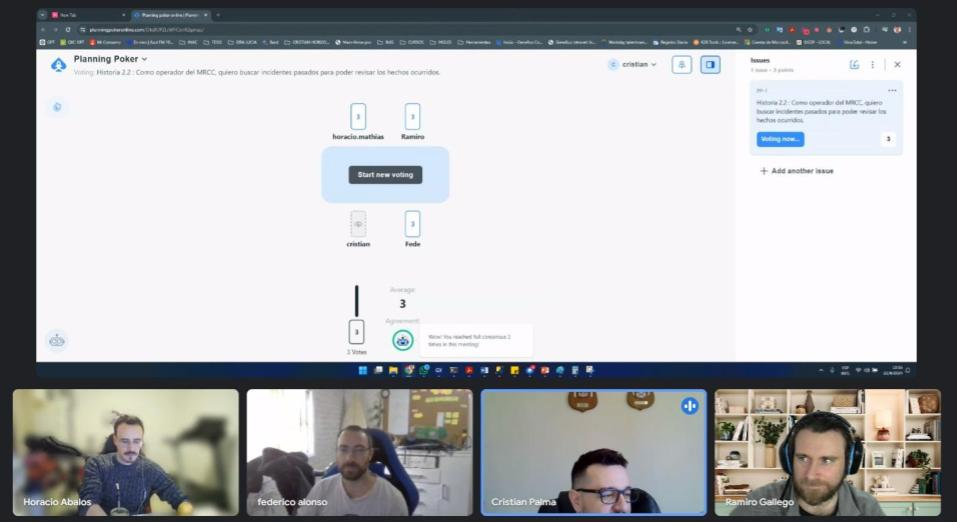
\includegraphics[width=0.8\textwidth]{../imagenes/secciones/4-Ingenieria-de-requerimientos/Poker Planning.jpg}
    \caption{Estimación de historias de usuario con Planning Poker}
    \label{fig:estimacionPokerPlanning}
\end{figure}


\subsection{Product backlog}

A continuación, se muestra un listado que incluye de forma resumida, todas las historias de usuario definidas por el equipo: